\chapter{水下图像多模态转译模型设计}
基于上述几章的分析,我们了解到水下图像合成的方法,一种是基于水下光学物理模型将给定图像合成水下场景图像,另一种是利用CycleGAN这种无监督图像转译模型,实现图像从当前场景到水下场景的转译。这些方法都无法一次生成多种样式的合成结果。将有限的给定输入图像,转译成多种水下环境条件的图像结果就显得尤为重要。

在上一章最后一小节,我们根据问题设计了两种思路,针对设想的两种思路给出具体的定义和分析,以及具体网络设计。

\section{水下图像跨域多模态转译设计}
% 定义、选择的baselines与问题之间的关系

我们将这种给定图像转译到多种水下环境的图像转译称作水下图像多模态转译。基于生成对抗网络,我们的网络结构可以在无监督条件下,实现水下图像的多模态转译
在上一章最后一小节,我们根据问题设计了两种思路,针对设想的两种思路给出具体的定义和分析,以及具体网络设计。

\subsection{问题及分析}
\subsection{模型创新点}
\subsection{目标函数和算法}
$A$域和$B$域分别为空中域和水下多模态域,给定图像$x_A \in A$和输入目标域风格随机采样编码$z_B$,我们训练从$A \rightarrow B$的方向上的转译,其中用到的目标函数如下所示。

\textbf{域对抗损失.} 训练过程中,翻译器网络输入纯净完整的内容信息和目标域风格信息,通过域对抗损失限制翻译器学习生成目标域结果

\begin{equation}
\label{equ:adv_a_}
L_{adv}^{\tilde{x}_A} = \mathbb{E}[\log D_A(x_A)] + \mathbb{E}[\log(1-D_A(G_A(c,s_A)))]
\end{equation}

\begin{equation}
\label{equ:adv_a}
L_{adv}^{\hat{x}_A} = \mathbb{E}[\log D_A(x_A)] + \mathbb{E}[\log(1-D_A(G_A(\hat{c},s_A)))]
\end{equation}

\begin{equation}
\label{equ:adv_b}
L_{adv}^{\hat{x}_B} = \mathbb{E}[\log D_B(x_B)] + \mathbb{E}[\log(1-D_B(G_B(c,z_B)))]
\end{equation}

生成器$G_A$学习使用来自$A$域的风格样式$s_A$生成$A$域具有足够真实性的图像$G_A(c,s_A)$和$G_A(\hat{c},s_A)$,企图可以混淆真实图像和生成结果,让$A$域判别器$D_A$无法区分他们。类似地,生成器$G_B$学习使用目标域分布采样编码$z_B$合成$B$域具有真实性的图像结果$G_B(c,z_B)$,目标也是让$B$域判别器$D_B$无法区分输入是真实图像还是生成假结果。

\textbf{循环一致性损失.}为了保证$A \rightarrow B$和$B \rightarrow A$两个方向上映射是循环一致的,我们使用CycleGAN~\cite{zhu2017unpaired}中提出的循环一致性损失来进行限制。

\begin{equation}
\label{equ:cycle}
L_{cyc} = \mathbb{E}[\| G_A(\hat{c}, s_A) - x_A \|_1]
\end{equation}

其中$G_A(\hat{c}, s_A)$是$x_A$的重建结果。

\textbf{Identity loss}. We adopt identity mapping between real sample and $G_A(c,s_A)$. 

\begin{equation}
\label{equ:idt}
L_{idt} = \mathbb{E}[\| G_A(c, s_A) - x_A \|_1]
\end{equation}

When encoders successfully disentangle input sample image into content and style parts, the distance between real sample and $G_A(c,s_A)$ is very small in theory.

\textbf{Content-consistent loss}.
To keep the content from source image unchanged between cross-domain translation, not only real image and the generated image but also the disentangled content codes $c$ and $\hat{c}$ from them should be consistent.

\begin{equation}
\label{equ:cc}
\begin{aligned}
L_{cc} & = \mathbb{E}[\| E_C(G_A(c, s_A)) - E_C(x_A) \|_1] \\
       & = \mathbb{E}[\| \hat{c} - c \|_1]
\end{aligned}
\end{equation}

\textbf{KL loss}. The KL loss L aims to align the representation of disentangled content and style with a prior Gaussian distribution.

\textbf{Full objective.}
Our full objective functions can be summarized as follows:
\begin{equation}
\label{equ:full}
\begin{aligned}
\min_{E,G}\max_{D} & L_{adv}^{\tilde{x}_A}+L_{adv}^{\hat{x}_A}+L_{adv}^{\hat{x}_B} \\
+&\lambda_{cyc}L_{cyc}+\lambda_{idt}L_{idt}+\lambda_{cc}L_{cc}+\lambda_{kl}L_{kl}
\end{aligned}
\end{equation}

where $\lambda_{cyc}$, $\lambda_{idt}$, $\lambda_{cc}$ and $\lambda_{kl}$ are hyperparameters for each term. We also further test our model using reference images instead of latent vectors when generating style codes. We set these parameters to $10$, $5$, $1$, $0.01$ by default.

\subsection{网络结构}

\begin{figure*}[ht]
    \centering
    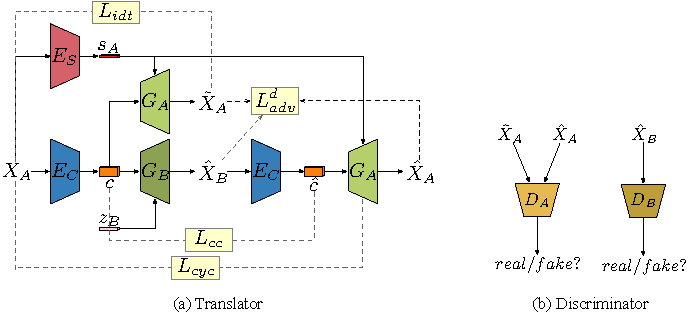
\includegraphics[width=1\textwidth]{figures/MUGAN.pdf}
    \caption{Caption}
    \label{fig:my_label}
\end{figure*}

\section{水下图像多样式域转译设计}

\subsection{问题及分析}
\subsection{模型创新点}
\subsection{目标函数和算法}
\subsection{网络结构}


\section{建立模型算法和损失函数}
\subsection{模型创新点}
\subsection{目标函数和算法}
\subsection{网络结构}


% \section{实验与分析}
% \subsection{数据集设置与实验环境}
% \subsection{评价指标}
% \subsection{消融实验}
% \subsection{与先进方法对比}

\section{本章小结}
